\documentclass{article}
\usepackage[utf8]{inputenc}
\usepackage[czech]{babel}
\usepackage{multirow}
\usepackage{tikz}
\usepackage{lscape}
\usepackage{rotating}
\usepackage{graphicx}
\graphicspath{ {./images/} }

\usepackage[%
    left=1.50in,%
    right=1.50in,%
    top=1.0in,%
    bottom=1.0in,%
    paperheight=11in,%
    paperwidth=8.5in%
]{geometry}%

\setlength{\parskip}{\baselineskip}%
\setlength{\parindent}{0pt}%

\title{Dokument zadavatele \\ Sigma Male Flowers s.r.o.}
\author{Denis Akopyan, Jiří Otoupal, Sergei Naumenko, Oleg Veres, Jiří Vrba}
\date{4IT216 - ZS 2021/2022}

\begin{document}

\maketitle
\clearpage

\section*{Charakteristika firmy}

Firma Sigma Male Flowers s.r.o. (také jako $\Sigma$ Male Flowers) podniká v České republice od roku 2010.
Má momentálně 2 pobočky/prodejny, jednu v Praze a jednu v Brně.
Firma má dohromady přibližně 30 zaměstnanců, s tím, že stálých zaměstnanců je tam přibližně 20, zbytek
jsou brigádnící a pracovníci na DPP, DPČ.

Ve firmě pracuje několik typů pracovníků: floristé, zákaznická podpora, kurýři a oddělení logistiky.

Firma nakupuje květiny levně na burzách v Holandsku a následně si objednává jejich dopravu do České Republiky a zde je prodává s marží. Díky levné nákupní ceně mohou pořádat speciální akce a prodávat květiny levněji než většina konkurence.

Firma provozuje jak kamenné prodejny, kde si mohou zákazníci z ulice zakoupit květiny bez předchozího objednání, tak e-shop, kde je možné si objednat květiny a následně si je buď nechat dovézt nebo si je vyzvednout osobně.
Firma také spolupracuje s rozvážkovou službou DámeKytky.cz s.r.o. která pro ně zajišťuje objednávání a následný rozvoz květin po Praze.
Rozvoz je v rámci celé České Republiky do 24 hodin a za poplatek, v případě Brna a Prahy pak do 6 hodin od objednání a zdarma.

Aby bylo možné květiny uchovávat, provozují obě položky sklad se sníženou teplotou.
Je potřeba evidovat, jaké a kolik květin se v každém skladu nachází, aby bylo možné včas nakoupit docházející druh v požadovaném množství.
K tomu slouží sdílená Excel tabulka, do které zapisují zaměstnanci floristé odpisy při vyřizování objednávek a naopak zaměstnanci z oddělení logistiky zapisují přírůstky množství jednotlivých typů při převzetí objednávky.

Všechny objednávky (jak z e-shopu a DámeKytky.cz, tak od zákazníků v kamenné prodejně) se zapisují do hromadné sdílené Excel tabulky, aby pak bylo možné objednávky vyřizovat floristy a následně je zahrnout do účetnictví.

Na základě objednávek pak pracovníci z oddělení marketingu ručně hledají vzory chování, aby mohli zvyšovat efektivitu budoucích marketingových kampaní. Celkově má firma velký potenciál pro těžbu znalostí ze svých dat.

Floristé potřebují vědět, jaké objednávky mají vázat z jakého množství květin.
Objednávky se vyřizují prioritně podle času vyzvednutí / předání kurýrovi a podle velikosti objednávky.
Objednávky s větším počtem květů se vyřizují přednostně před objednávkami s malým počtem.

Zákaznická podpora zpracovává dotazy od uživatelů e-shopu, komunikuje s nimi v reálném čase pomocí chatu a přijímá objednávky po telefonu.

Kurýři rozvážejí objednávky a potřebují znát optimalizované trasy (v ideálním případě všechny objednávky v jedné lokalitě rozvážet najednou)

Pracovníci logistiky plánují trasy kurýrů, zajišťují zásoby zboží na skladě, v případě potřeby vytváří objednávky u obchodníků na Holandské burze a zajišťují dopravu do České Republiky.

\section*{Vize}

Firma má v plánu do budoucna expandovat pole svojí působnosti do dalších částí České Republiky
a otevřít nové pobočky v Ostravě, Plzni a Liberci. Dále má v plánu zvyšovat objem objednávek a tím
pádem i zvýšit svůj obrat a zisky z přidané marže.

K tomu, aby byla firma schopná expandovat potřebuje ale investovat do IT a potřebuje centrální systém, protože bez něj by bylo velice obtížné zvládat nárůst administrační a logistické zátěže.

Momentální stav IT ve firmě neumožňuje být dostatečně flexibilní a je jedním z hlavních faktorů bránící rozvoji.

Firma má také do budoucna plány zefektivnit svůj proces příjmání nových zaměnstnanců a management brigádníků v období nadměrného zatížení (např. Den matek nebo svátek sv. Valentýna, kdy vytíženost firmy přesahuje několikanásobně průměr)

\section*{Poslání}

Posláním společnosti je zpřístupnit široké veřejnosti květiny vysoké kvality, ale zároveň zachovat nízkou cenu.
Společnost se snaží cílit na velice obsáhlou cílovou skupinu, ale zároveň se snaží posílit svojí pozici na trhu s květinami pomocí speciálně cílených marketingových kampaní. V České Republice je vysoká konkurence a proto je potřeba pečlivě volit prodejní strategii a stanovování cen.

\clearpage


\section*{SWOT Analýza společnosti}

SWOT analýza je jednou z nejčastějších metod strategické analýzy.
Skládá se ze čtyř částí:
\begin{itemize}
    \item \textbf{S}trenghts - silné stránky společnosti
    \item \textbf{W}eaknesses - slabé stránky společnosti
    \item \textbf{O}pportunities - potencionální příležitosti
    \item \textbf{T}hreats - hrozby pro společnost
\end{itemize}

\begin{table*}[h]
    \begin{tabular}{|p{195pt}|p{195pt}|}
        \hline \bfseries Strengths &\bfseries Weaknesses  \\
        \hline
        {\begin{itemize}
            \item Kvalifikovaný personál floristů
            \item Kvalita produktu
            \item Individuální přístup k zákazníkům
            \item Stabilní supply chain + distribuce
        \end{itemize}}
        &
        {\begin{itemize}
            \item Nízké povědomí o firmě
            \item Prodej zboží s nízkou trvanlivostí
            \item Vysoké náklady na skladování
            \item Závislost na ekologických faktorech
            \item Informační šum mezi zaměstnanci
        \end{itemize}} \\
        \hline \bfseries Opportunities &\bfseries Threats  \\
        \hline
        {\begin{itemize}
            \item Květinové dekorace na oslavy a svatby
            \item Propojení s jinýmy službami poskytující rozvoz (Messenger, Bolt)
            \item Flower mystery boxes
        \end{itemize}} &
        {\begin{itemize}
            \item Vstup nové konkurence
            \item Upadající zájem ze strany zákazníků
            \item Legislativní změny (např. clo)
            \item Administrativní náročnost
        \end{itemize}} \\
        \hline
    \end{tabular}
\end{table*}

\section*{Byznys cíle společnosti}
\begin{itemize}
    \item Zvýšit podíl na českém trhu s květinami z 5\% na 16\% v průběhu maximálně 2 let
    \item Zvýšit efektivitu produkce a snížit čas potřebný na vyřízení objednávky o 10\%
    \item Zlepšit flexibilitu společnosti - snížit administrativní náklady a čas potřebný k náboru nových zaměstnanců o 30\%
    \item Zvýšit kapacitu objednávek o 20\% do konce roku 2022
    \item Rozšířit firmu o 1 pobočku do konce roku 2023 a o další 2 pak do 3 let
\end{itemize}

\clearpage

\section*{Business Model Canvas}
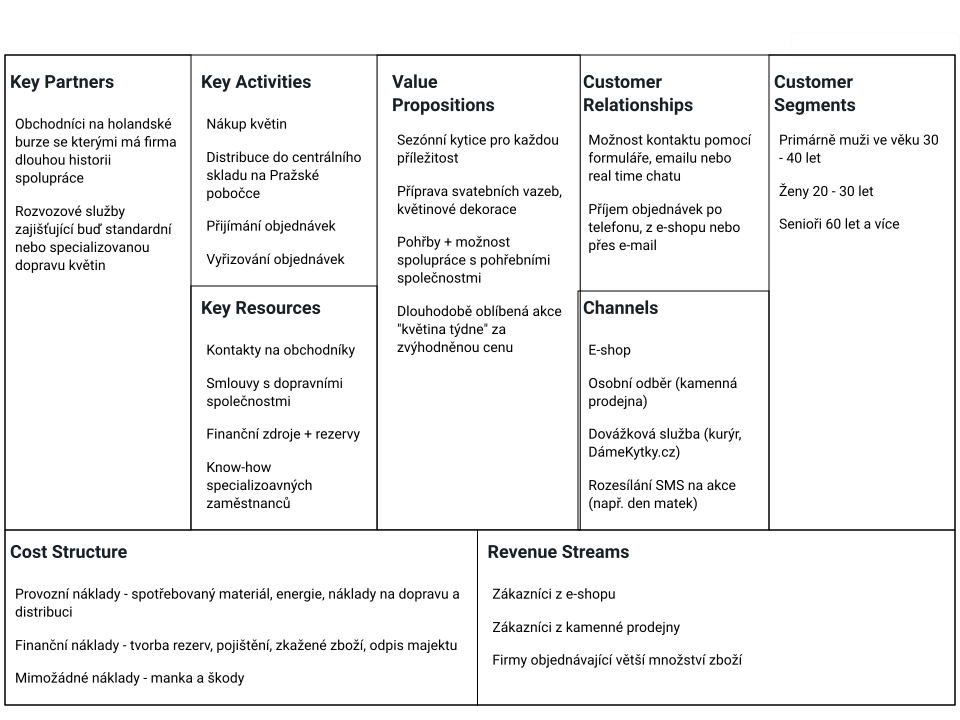
\includegraphics[width=\linewidth]{images/bmc.png}

\newpage

\section*{Popis současného stavu}

\subsection*{Procesy ve firmě}

\begin{figure}[h]
\caption{Objednávka květin na Holandské burze + vytvoření objednávky u dodavatele}
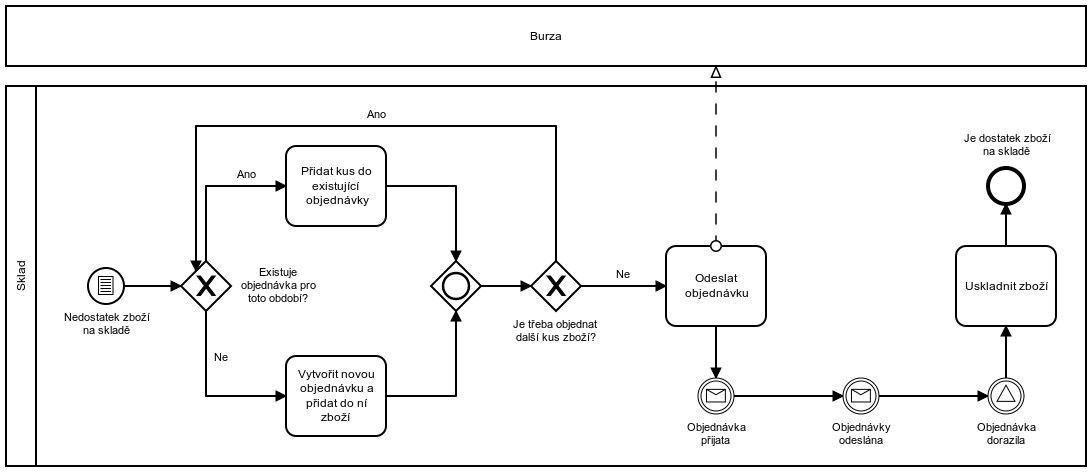
\includegraphics[width=\linewidth]{images/procesy/1.png}
\end{figure}

\newpage
\begin{figure}[h]
\caption{Doprava zboží z Holandska do České Republiky}
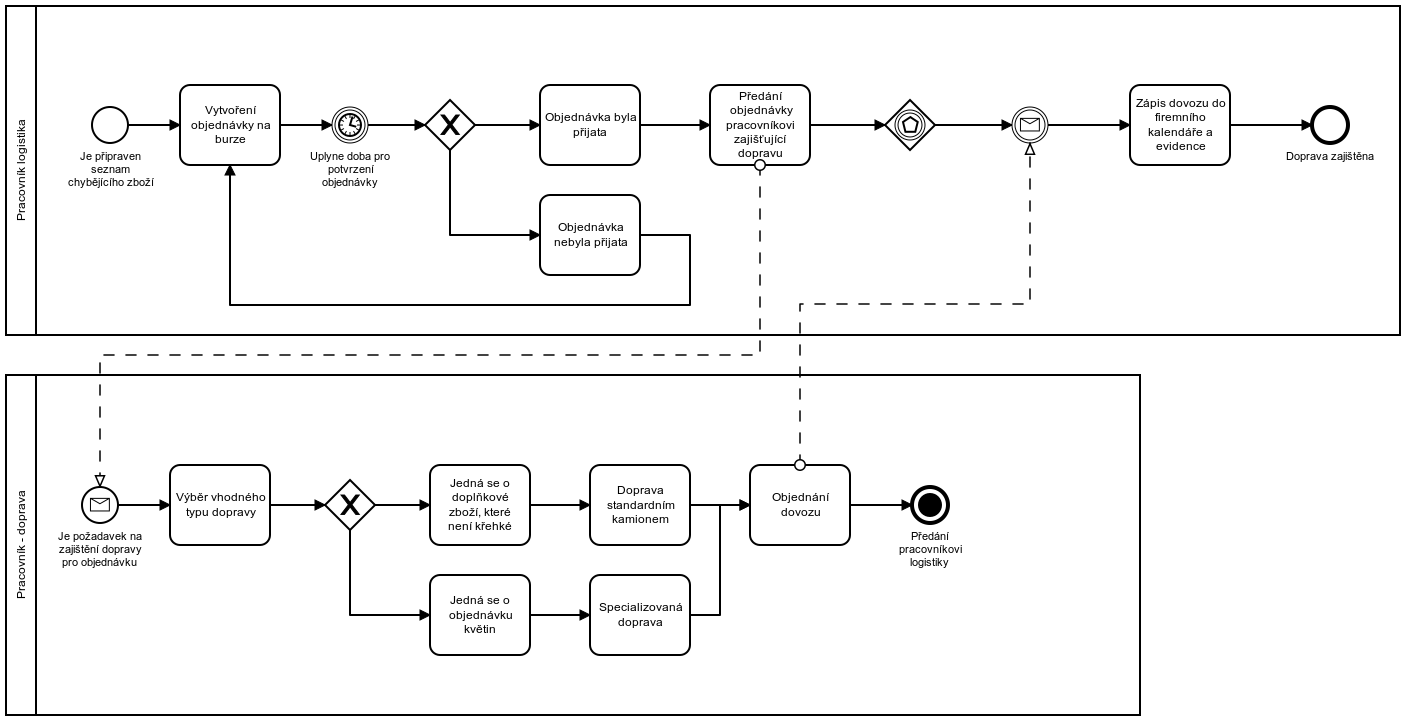
\includegraphics[width=\linewidth]{images/procesy/2.png}
\end{figure}

\newpage
\begin{figure}[h]
\caption{Distribuce zboží do ostatních poboček}
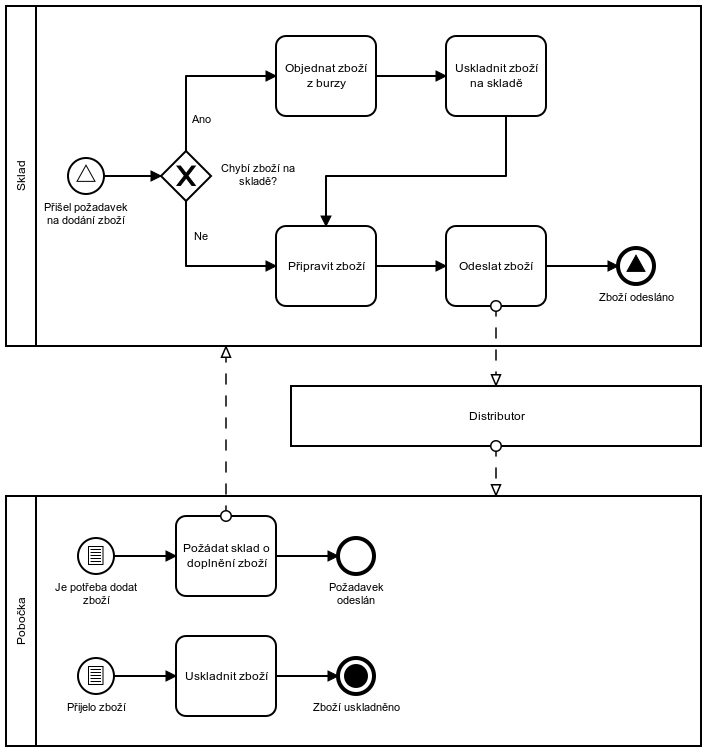
\includegraphics[width=\linewidth]{images/procesy/3.png}
\end{figure}

\newpage
\begin{figure}[h]
\caption{Vytvoření objednávky v kamenném obchodě}
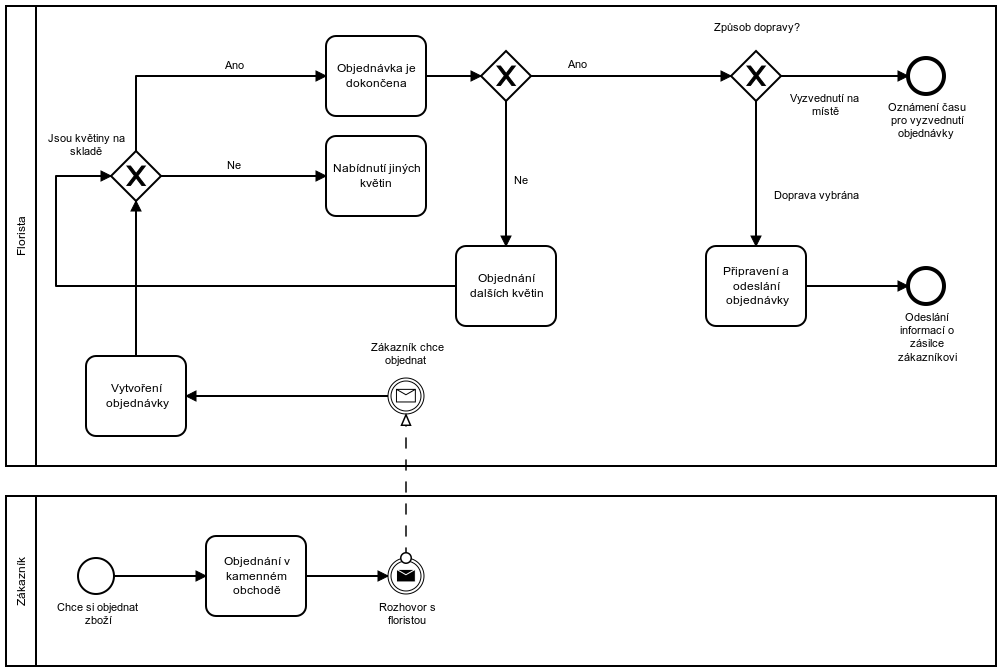
\includegraphics[width=\linewidth]{images/procesy/4.png}
\end{figure}

\newpage
\begin{figure}[h]
\caption{Vytvoření objednávky na e-shopu}
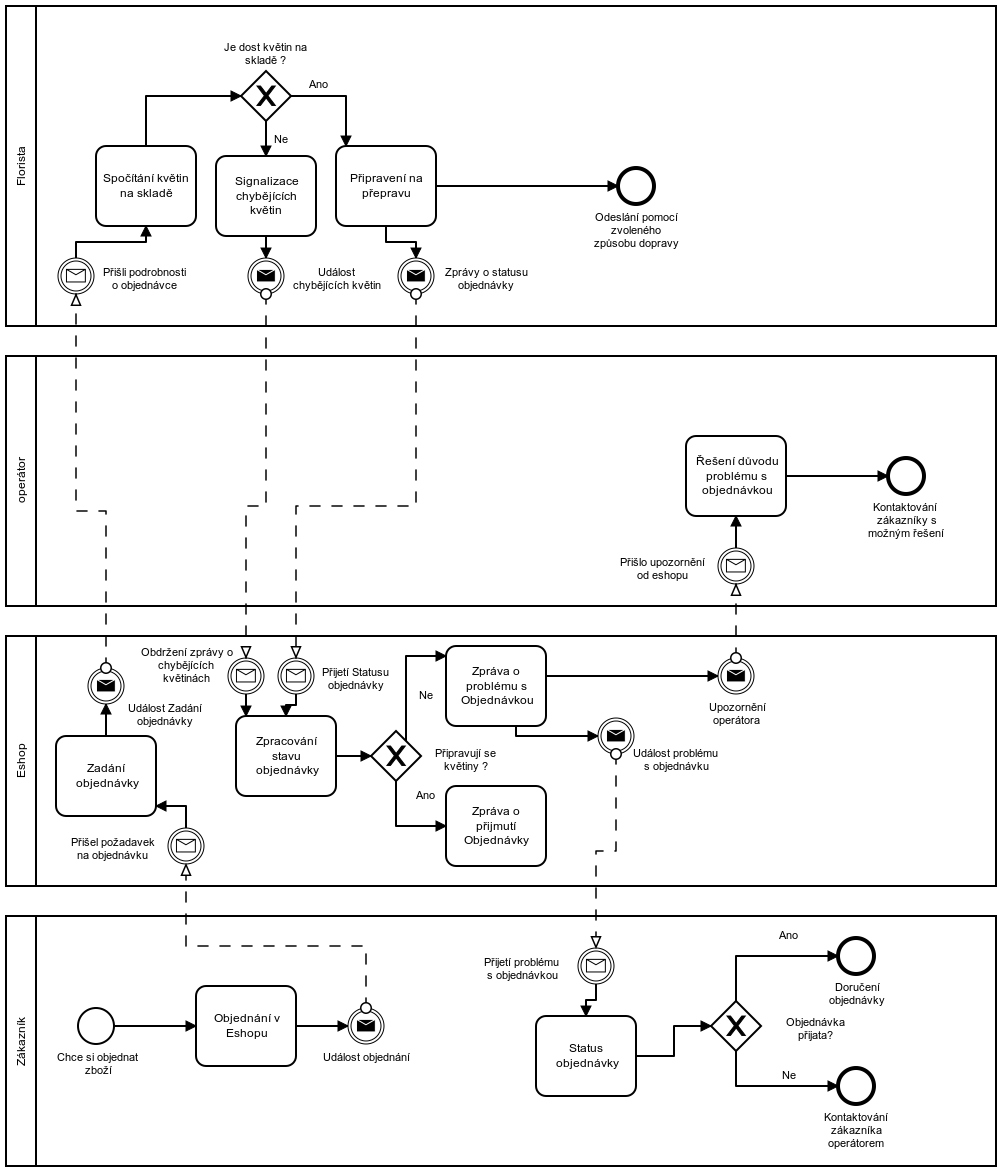
\includegraphics[width=\linewidth]{images/procesy/5.png}
\end{figure}

\newpage
\begin{figure}[h]
\caption{Vytvoření objednávky přes telefon}
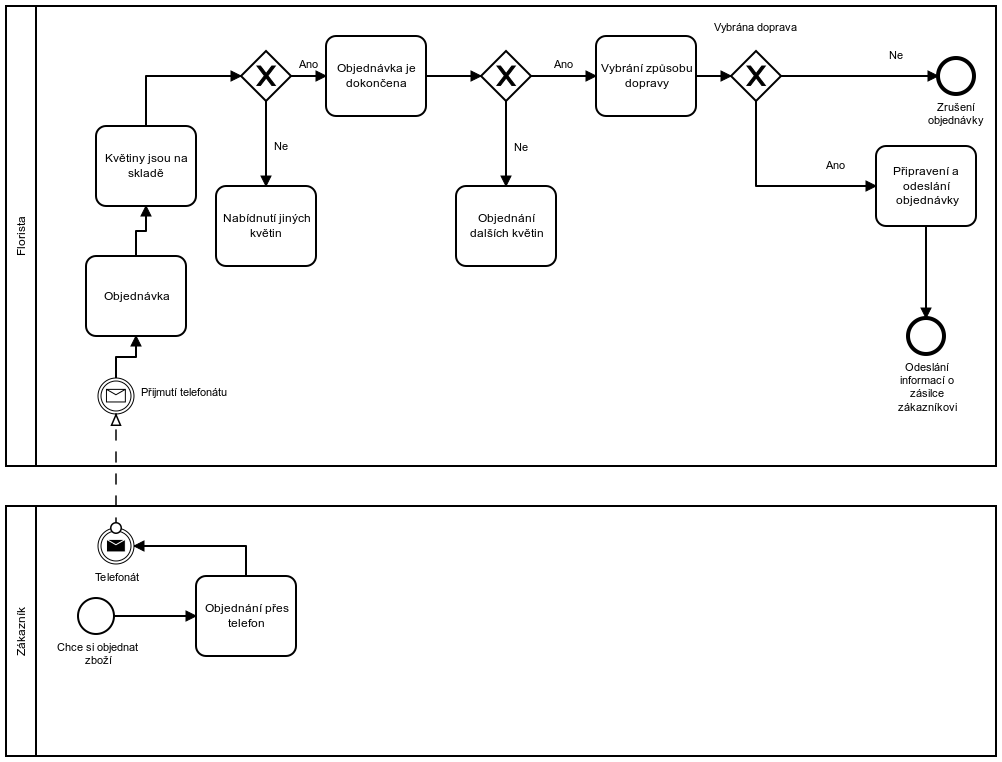
\includegraphics[width=\linewidth]{images/procesy/6.png}
\end{figure}

\newpage
\begin{figure}[h]
\caption{Vytvoření objednávky přes on-line službu (damekytky.cz)}
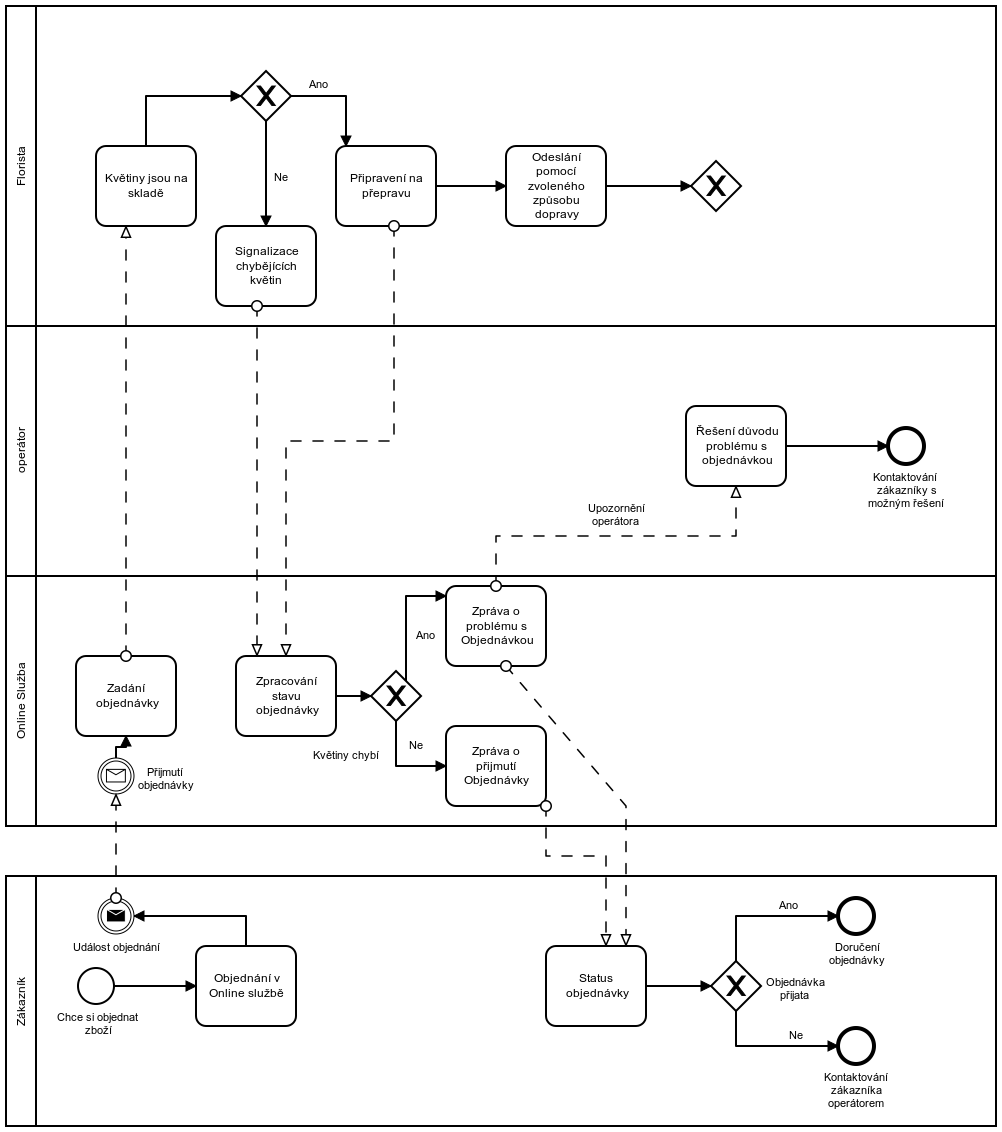
\includegraphics[width=\linewidth]{images/procesy/7.png}
\end{figure}

\newpage
\begin{figure}[h]
\caption{Příprava objednávky floristou}
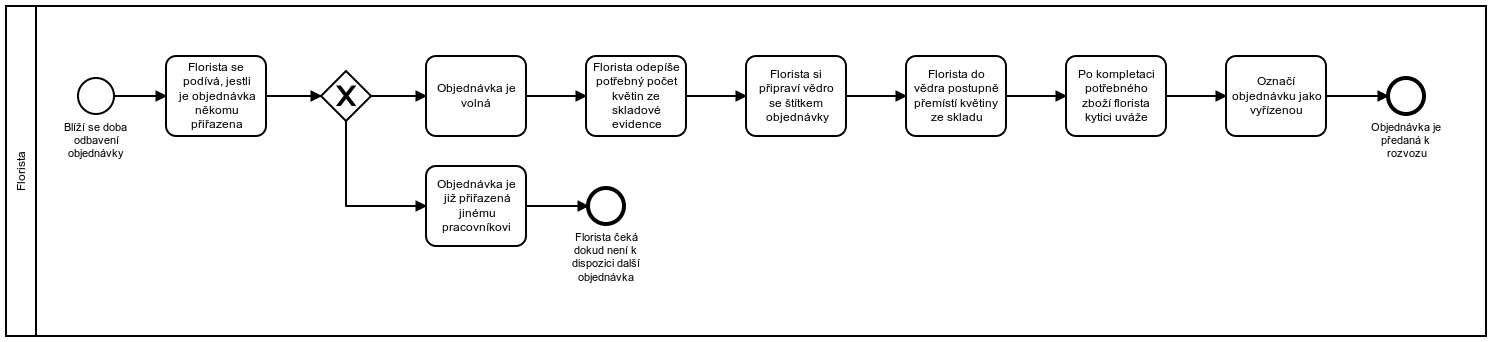
\includegraphics[width=\linewidth]{images/procesy/8.png}
\end{figure}

\newpage
\begin{figure}[h]
\caption{Distribuce připravené objednávky k zákazníkovi}
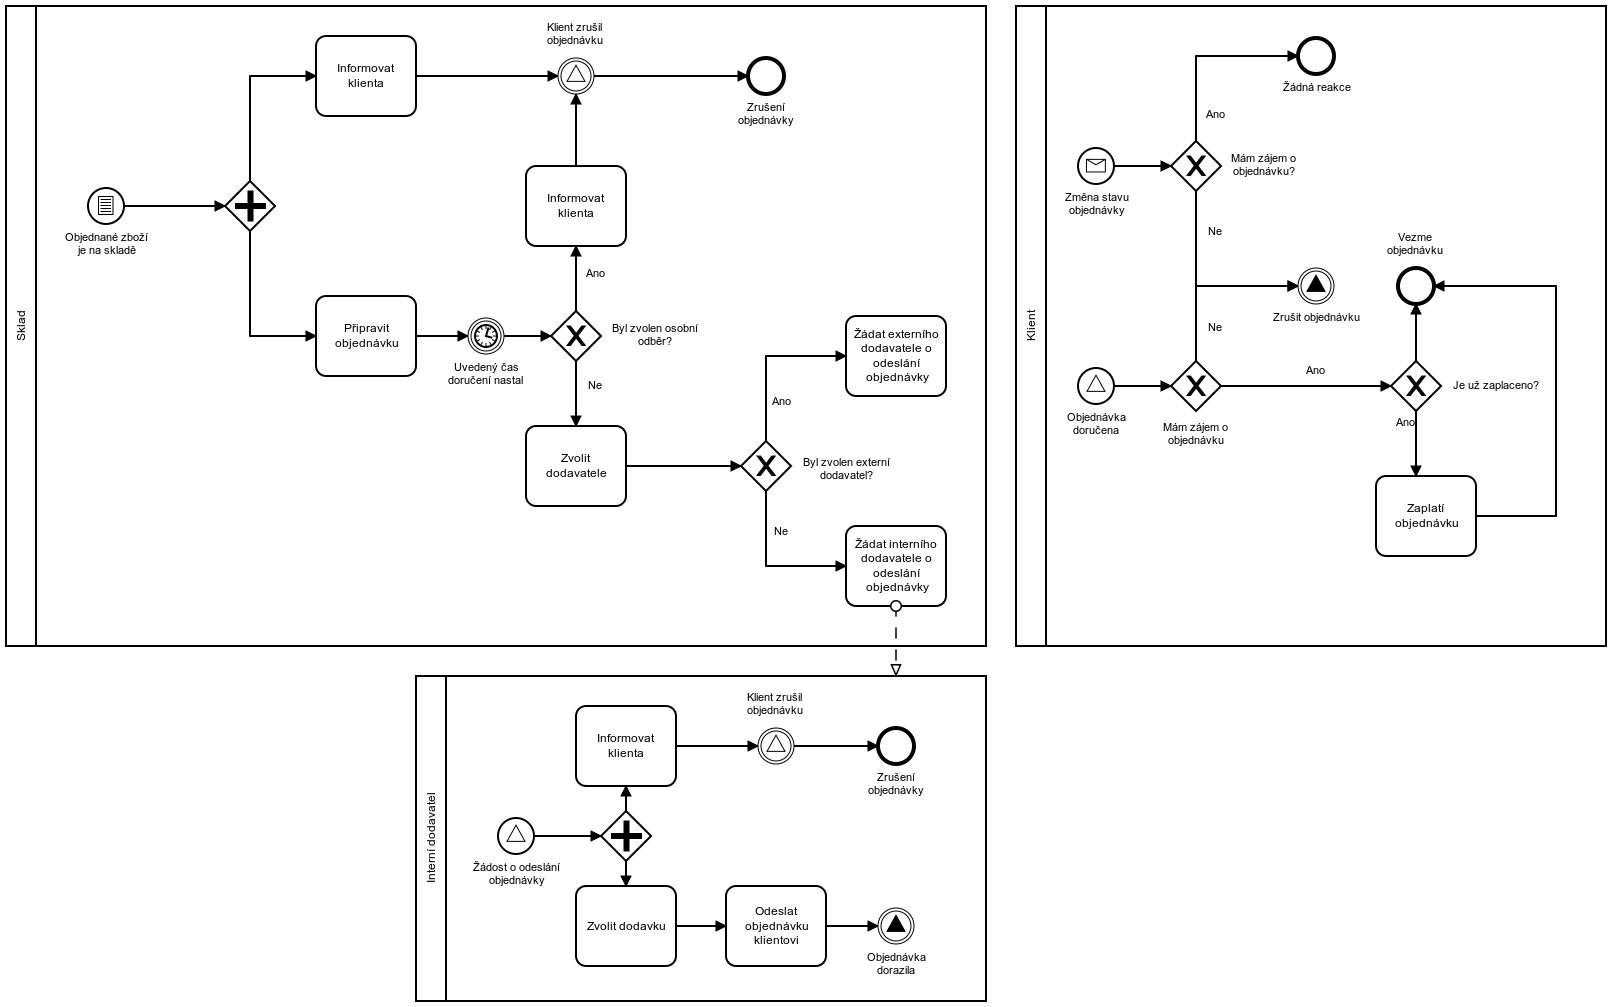
\includegraphics[width=\linewidth]{images/procesy/9.png}
\end{figure}

\newpage
\begin{figure}[h]
\caption{Reklamace při vyzvednutí osobně}
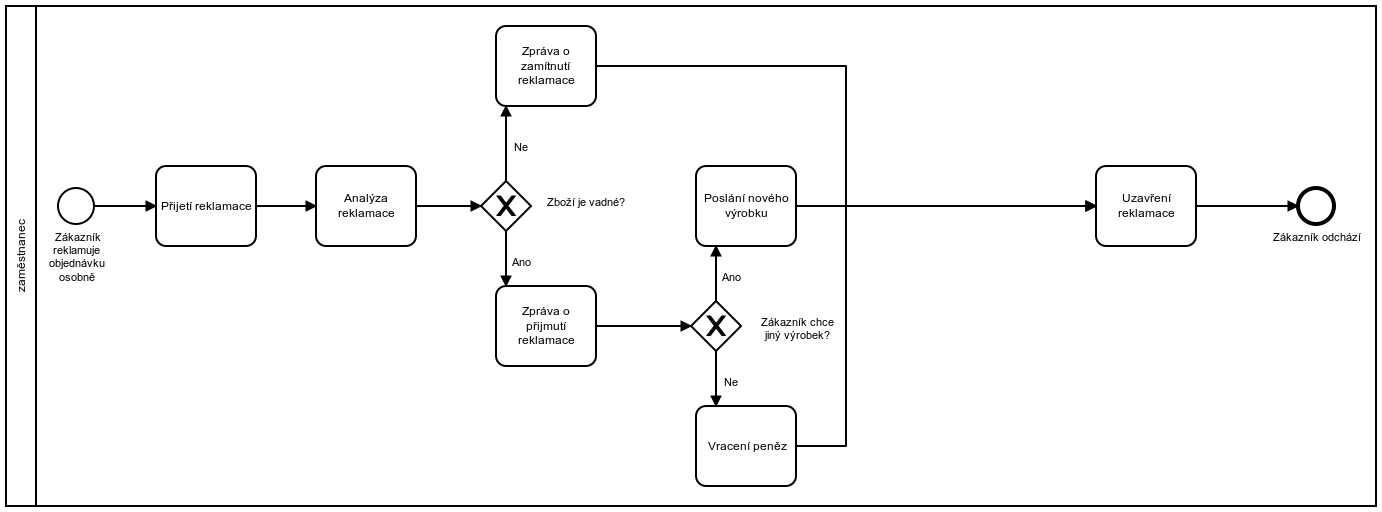
\includegraphics[width=\linewidth]{images/procesy/10.png}
\end{figure}

\newpage
\begin{figure}[h]
\caption{Reklamace objednávky při doručení kurýrem}
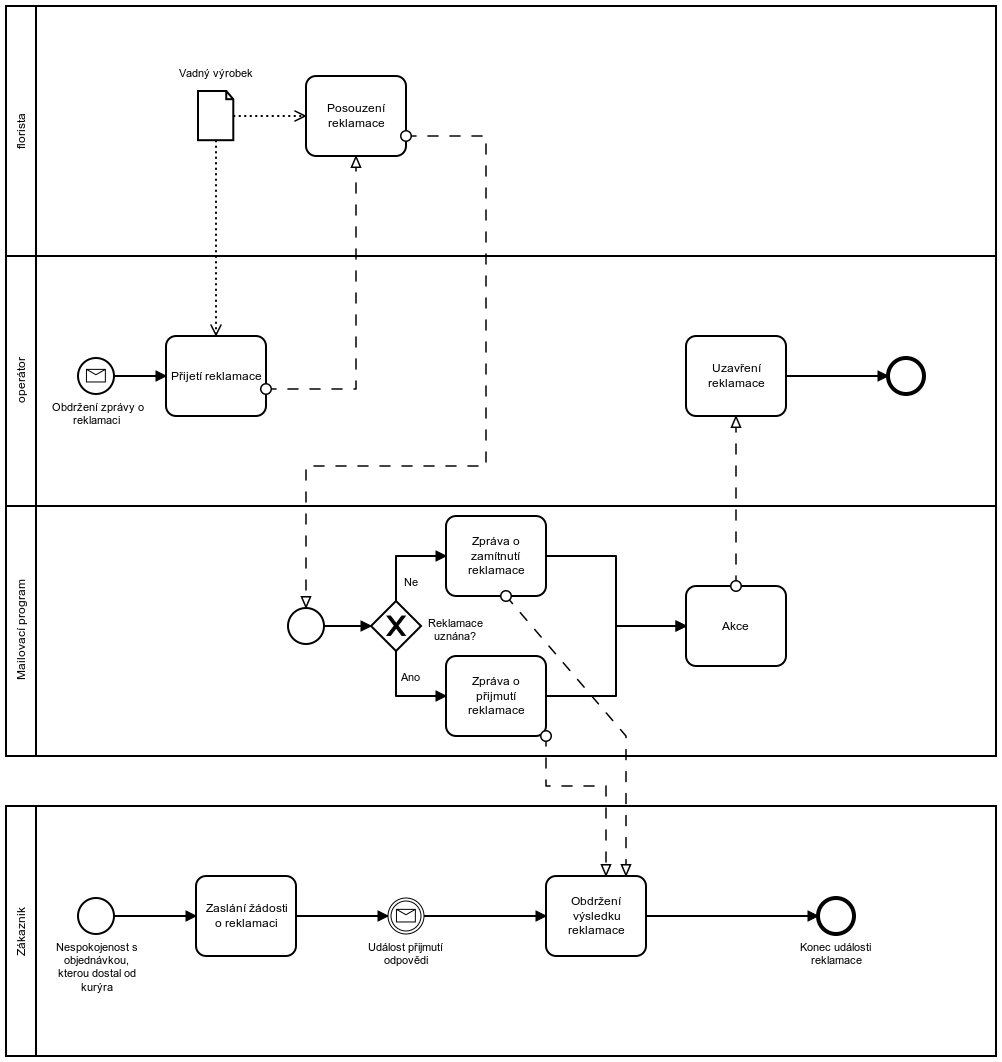
\includegraphics[width=\linewidth]{images/procesy/11.png}
\end{figure}

\newpage
\begin{figure}[h]
\caption{Sdílení reklamy}
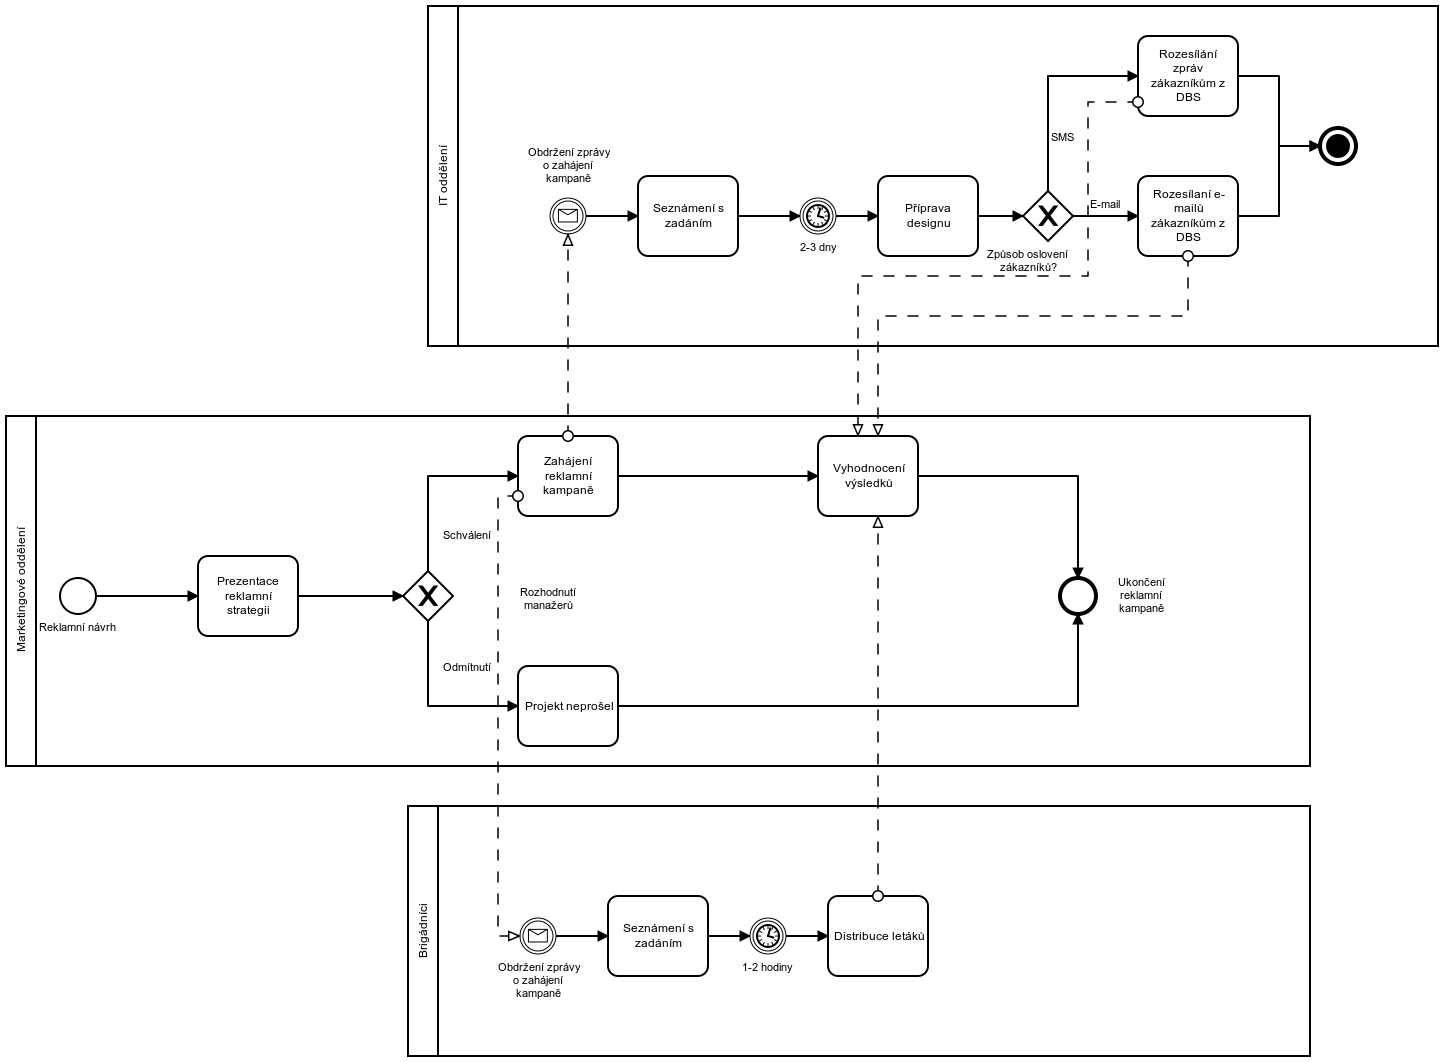
\includegraphics[width=\linewidth]{images/procesy/12.png}
\end{figure}

\newpage
\begin{figure}[h]
\caption{Kontrola zboží + přijetí zboží na pobočce}
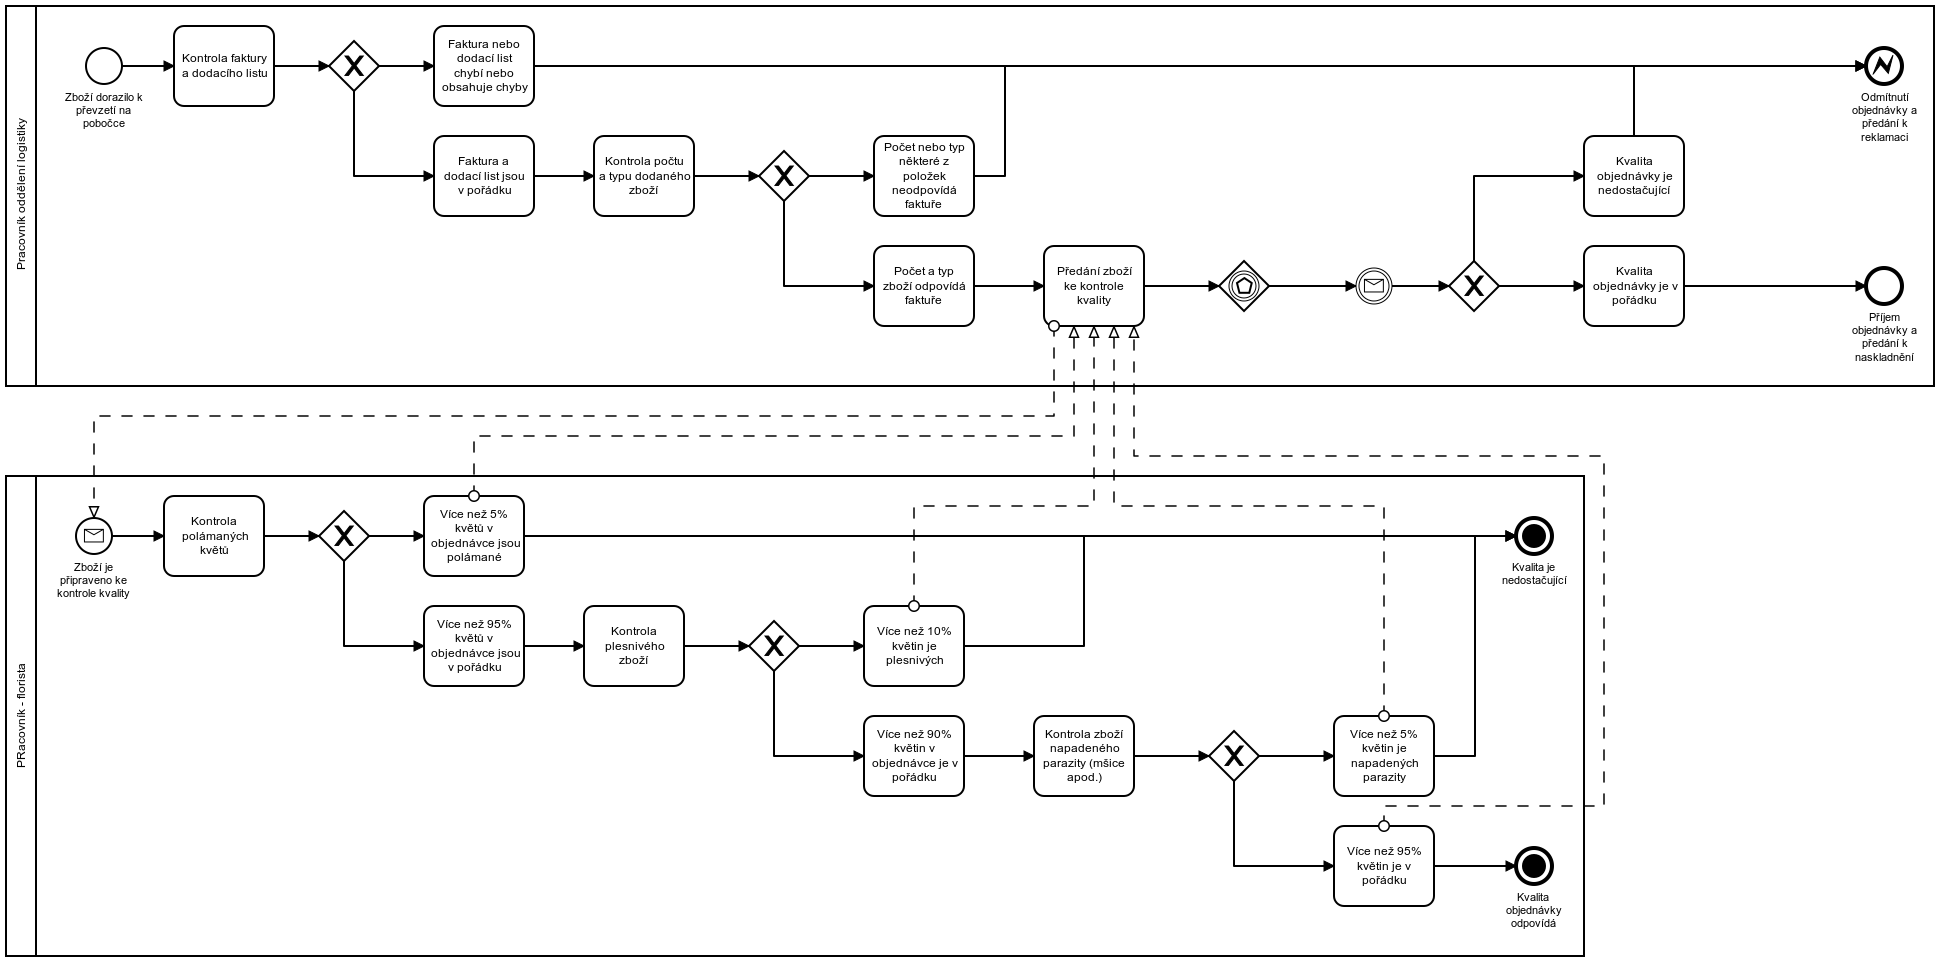
\includegraphics[width=\linewidth]{images/procesy/13.png}
\end{figure}


\newpage
\begin{figure}[h]
\caption{Plánování směn zaměstnanců}
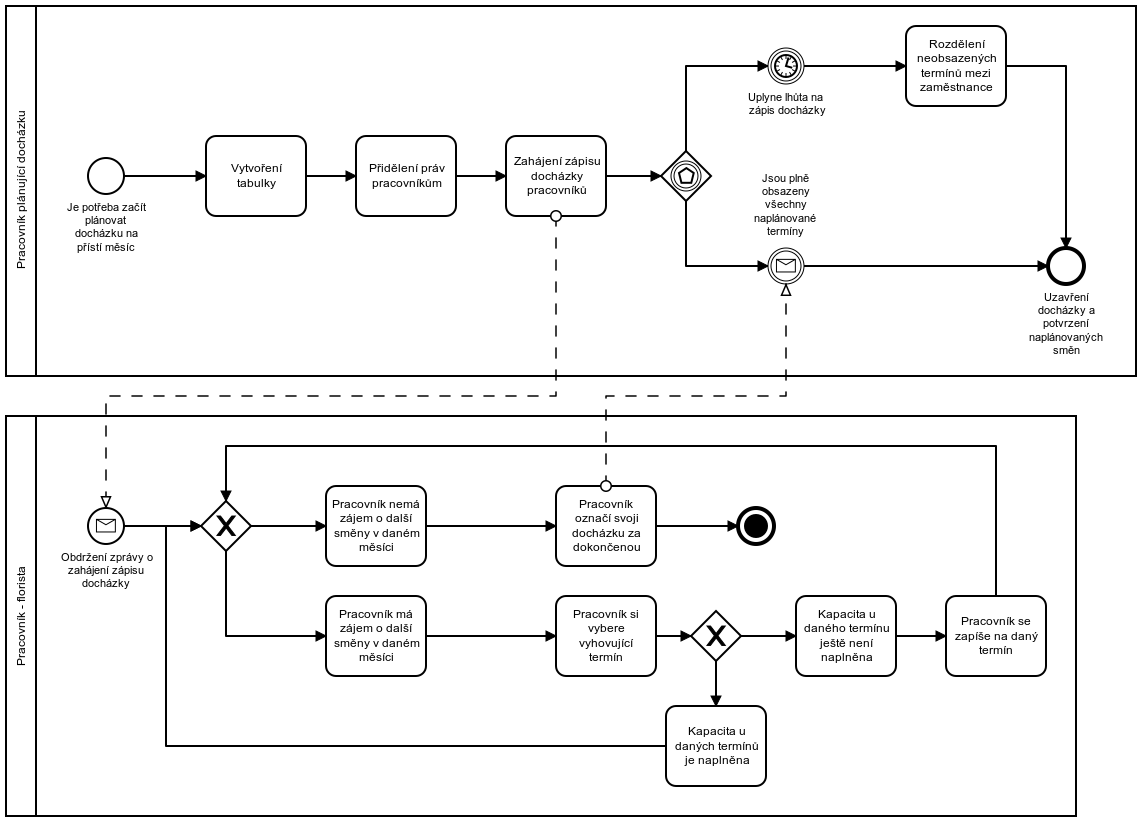
\includegraphics[width=\linewidth]{images/procesy/14.png}
\end{figure}

\newpage
\begin{figure}[h]
\caption{Uskladnění zboží + zadání do skladové evidence}
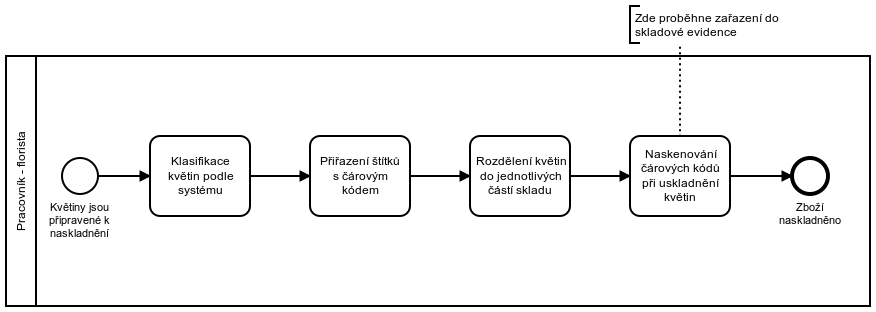
\includegraphics[width=\linewidth]{images/procesy/15.png}
\end{figure}

\newpage
\begin{figure}[h]
\caption{Vyřazení zkaženého zboží ze skladu}
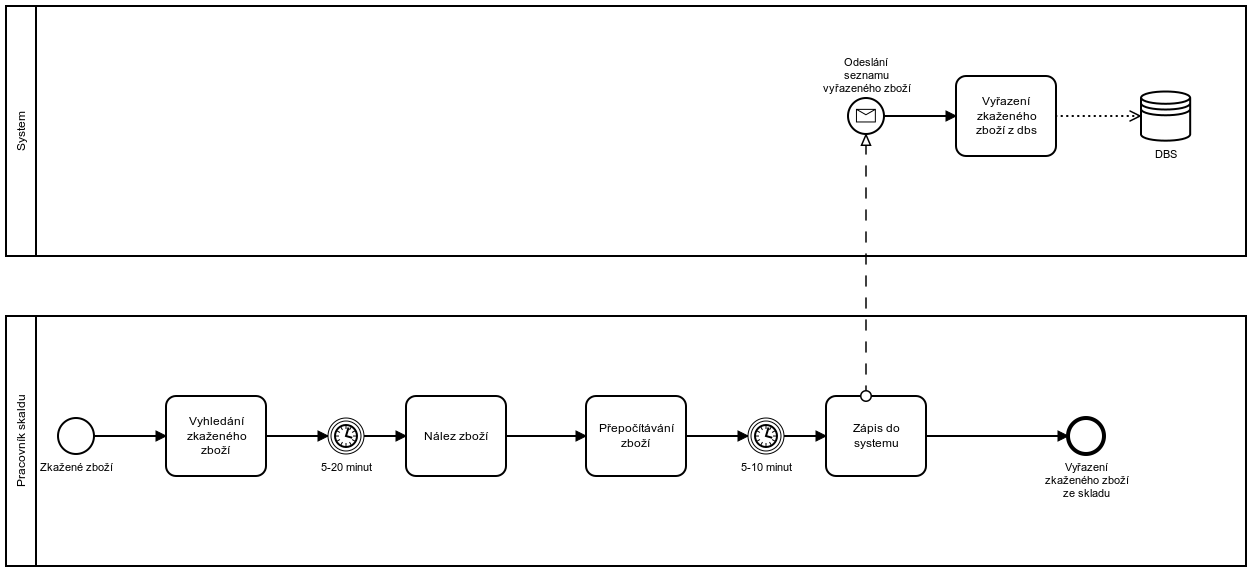
\includegraphics[width=\linewidth]{images/procesy/16.png}
\end{figure}

\newpage
\begin{figure}[h]
\caption{Ošetření květin před naskladněním}
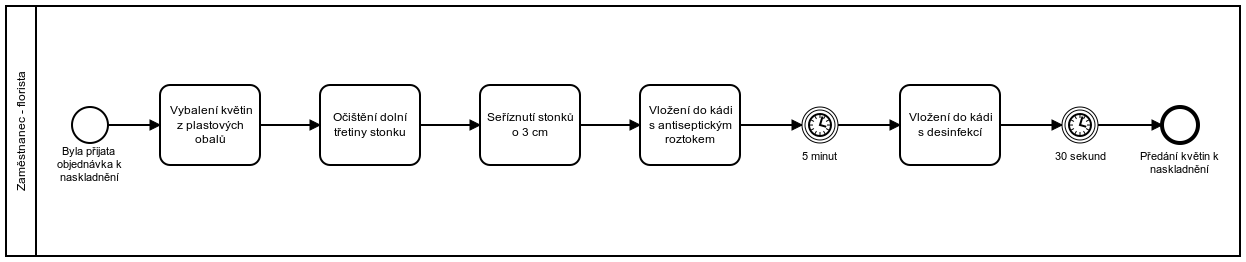
\includegraphics[width=\linewidth]{images/procesy/17.png}
\end{figure}

\newpage
\begin{figure}[h]
\caption{Zajištění komunikace se zákazníkem ohledně stavu objednávky}
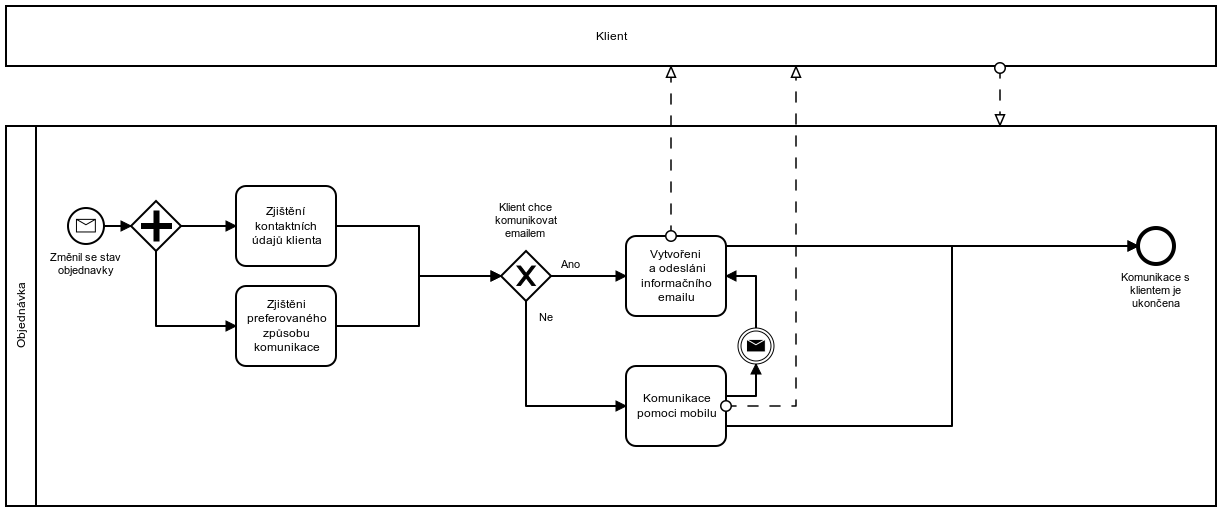
\includegraphics[width=\linewidth]{images/procesy/18.png}
\end{figure}

\newpage
\begin{figure}[h]
\centering
\caption{Real time komunikace s uživatelem e-shopu (chat)}
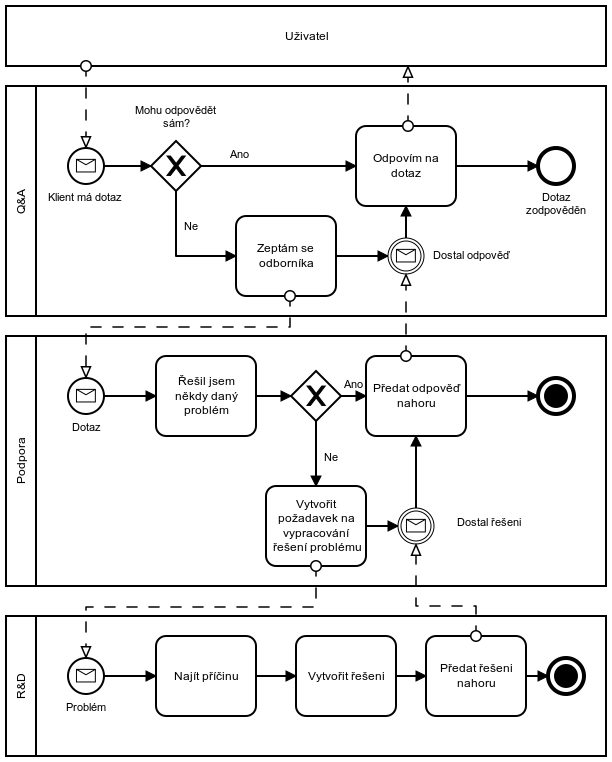
\includegraphics[width=\dimexpr\linewidth-50pt\relax]{images/procesy/19.png}
\end{figure}

\newpage
\begin{figure}[h]
\caption{Hiring nových zaměstnanců}
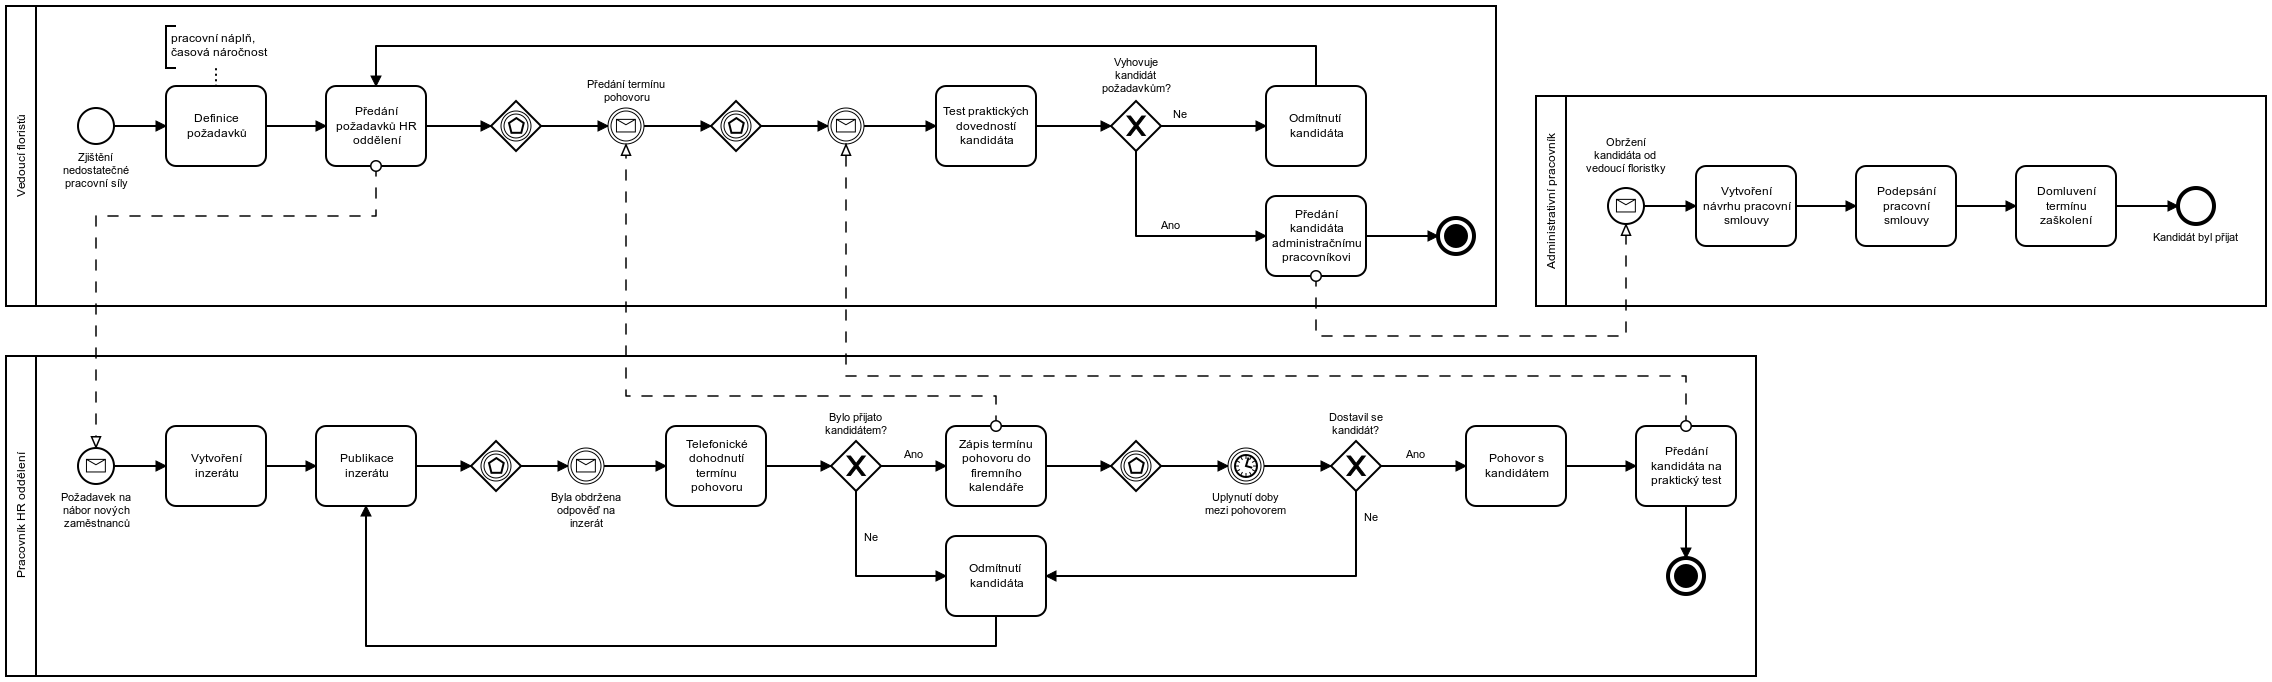
\includegraphics[width=\linewidth]{images/procesy/20.png}
\end{figure}

\newpage

\subsection*{Souhrnná analýza stavu IT}

\end{document}
